
% Default to the notebook output style

    


% Inherit from the specified cell style.




    
\documentclass{article}

    
    
    \usepackage{graphicx} % Used to insert images
    \usepackage{adjustbox} % Used to constrain images to a maximum size 
    \usepackage{color} % Allow colors to be defined
    \usepackage{enumerate} % Needed for markdown enumerations to work
    \usepackage{geometry} % Used to adjust the document margins
    \usepackage{amsmath} % Equations
    \usepackage{amssymb} % Equations
    \usepackage{eurosym} % defines \euro
    \usepackage[mathletters]{ucs} % Extended unicode (utf-8) support
    \usepackage[utf8x]{inputenc} % Allow utf-8 characters in the tex document
    \usepackage{fancyvrb} % verbatim replacement that allows latex
    \usepackage{grffile} % extends the file name processing of package graphics 
                         % to support a larger range 
    % The hyperref package gives us a pdf with properly built
    % internal navigation ('pdf bookmarks' for the table of contents,
    % internal cross-reference links, web links for URLs, etc.)
    \usepackage{hyperref}
    \usepackage{longtable} % longtable support required by pandoc >1.10
    \usepackage{booktabs}  % table support for pandoc > 1.12.2
    

    
    
    \definecolor{orange}{cmyk}{0,0.4,0.8,0.2}
    \definecolor{darkorange}{rgb}{.71,0.21,0.01}
    \definecolor{darkgreen}{rgb}{.12,.54,.11}
    \definecolor{myteal}{rgb}{.26, .44, .56}
    \definecolor{gray}{gray}{0.45}
    \definecolor{lightgray}{gray}{.95}
    \definecolor{mediumgray}{gray}{.8}
    \definecolor{inputbackground}{rgb}{.95, .95, .85}
    \definecolor{outputbackground}{rgb}{.95, .95, .95}
    \definecolor{traceback}{rgb}{1, .95, .95}
    % ansi colors
    \definecolor{red}{rgb}{.6,0,0}
    \definecolor{green}{rgb}{0,.65,0}
    \definecolor{brown}{rgb}{0.6,0.6,0}
    \definecolor{blue}{rgb}{0,.145,.698}
    \definecolor{purple}{rgb}{.698,.145,.698}
    \definecolor{cyan}{rgb}{0,.698,.698}
    \definecolor{lightgray}{gray}{0.5}
    
    % bright ansi colors
    \definecolor{darkgray}{gray}{0.25}
    \definecolor{lightred}{rgb}{1.0,0.39,0.28}
    \definecolor{lightgreen}{rgb}{0.48,0.99,0.0}
    \definecolor{lightblue}{rgb}{0.53,0.81,0.92}
    \definecolor{lightpurple}{rgb}{0.87,0.63,0.87}
    \definecolor{lightcyan}{rgb}{0.5,1.0,0.83}
    
    % commands and environments needed by pandoc snippets
    % extracted from the output of `pandoc -s`
    \DefineVerbatimEnvironment{Highlighting}{Verbatim}{commandchars=\\\{\}}
    % Add ',fontsize=\small' for more characters per line
    \newenvironment{Shaded}{}{}
    \newcommand{\KeywordTok}[1]{\textcolor[rgb]{0.00,0.44,0.13}{\textbf{{#1}}}}
    \newcommand{\DataTypeTok}[1]{\textcolor[rgb]{0.56,0.13,0.00}{{#1}}}
    \newcommand{\DecValTok}[1]{\textcolor[rgb]{0.25,0.63,0.44}{{#1}}}
    \newcommand{\BaseNTok}[1]{\textcolor[rgb]{0.25,0.63,0.44}{{#1}}}
    \newcommand{\FloatTok}[1]{\textcolor[rgb]{0.25,0.63,0.44}{{#1}}}
    \newcommand{\CharTok}[1]{\textcolor[rgb]{0.25,0.44,0.63}{{#1}}}
    \newcommand{\StringTok}[1]{\textcolor[rgb]{0.25,0.44,0.63}{{#1}}}
    \newcommand{\CommentTok}[1]{\textcolor[rgb]{0.38,0.63,0.69}{\textit{{#1}}}}
    \newcommand{\OtherTok}[1]{\textcolor[rgb]{0.00,0.44,0.13}{{#1}}}
    \newcommand{\AlertTok}[1]{\textcolor[rgb]{1.00,0.00,0.00}{\textbf{{#1}}}}
    \newcommand{\FunctionTok}[1]{\textcolor[rgb]{0.02,0.16,0.49}{{#1}}}
    \newcommand{\RegionMarkerTok}[1]{{#1}}
    \newcommand{\ErrorTok}[1]{\textcolor[rgb]{1.00,0.00,0.00}{\textbf{{#1}}}}
    \newcommand{\NormalTok}[1]{{#1}}
    
    % Define a nice break command that doesn't care if a line doesn't already
    % exist.
    \def\br{\hspace*{\fill} \\* }
    % Math Jax compatability definitions
    \def\gt{>}
    \def\lt{<}
    % Document parameters
    \title{\texttt{NumPy} Basics}
    
    
    

    % Pygments definitions
    
\makeatletter
\def\PY@reset{\let\PY@it=\relax \let\PY@bf=\relax%
    \let\PY@ul=\relax \let\PY@tc=\relax%
    \let\PY@bc=\relax \let\PY@ff=\relax}
\def\PY@tok#1{\csname PY@tok@#1\endcsname}
\def\PY@toks#1+{\ifx\relax#1\empty\else%
    \PY@tok{#1}\expandafter\PY@toks\fi}
\def\PY@do#1{\PY@bc{\PY@tc{\PY@ul{%
    \PY@it{\PY@bf{\PY@ff{#1}}}}}}}
\def\PY#1#2{\PY@reset\PY@toks#1+\relax+\PY@do{#2}}

\expandafter\def\csname PY@tok@gd\endcsname{\def\PY@tc##1{\textcolor[rgb]{0.63,0.00,0.00}{##1}}}
\expandafter\def\csname PY@tok@gu\endcsname{\let\PY@bf=\textbf\def\PY@tc##1{\textcolor[rgb]{0.50,0.00,0.50}{##1}}}
\expandafter\def\csname PY@tok@gt\endcsname{\def\PY@tc##1{\textcolor[rgb]{0.00,0.27,0.87}{##1}}}
\expandafter\def\csname PY@tok@gs\endcsname{\let\PY@bf=\textbf}
\expandafter\def\csname PY@tok@gr\endcsname{\def\PY@tc##1{\textcolor[rgb]{1.00,0.00,0.00}{##1}}}
\expandafter\def\csname PY@tok@cm\endcsname{\let\PY@it=\textit\def\PY@tc##1{\textcolor[rgb]{0.25,0.50,0.50}{##1}}}
\expandafter\def\csname PY@tok@vg\endcsname{\def\PY@tc##1{\textcolor[rgb]{0.10,0.09,0.49}{##1}}}
\expandafter\def\csname PY@tok@m\endcsname{\def\PY@tc##1{\textcolor[rgb]{0.40,0.40,0.40}{##1}}}
\expandafter\def\csname PY@tok@mh\endcsname{\def\PY@tc##1{\textcolor[rgb]{0.40,0.40,0.40}{##1}}}
\expandafter\def\csname PY@tok@go\endcsname{\def\PY@tc##1{\textcolor[rgb]{0.53,0.53,0.53}{##1}}}
\expandafter\def\csname PY@tok@ge\endcsname{\let\PY@it=\textit}
\expandafter\def\csname PY@tok@vc\endcsname{\def\PY@tc##1{\textcolor[rgb]{0.10,0.09,0.49}{##1}}}
\expandafter\def\csname PY@tok@il\endcsname{\def\PY@tc##1{\textcolor[rgb]{0.40,0.40,0.40}{##1}}}
\expandafter\def\csname PY@tok@cs\endcsname{\let\PY@it=\textit\def\PY@tc##1{\textcolor[rgb]{0.25,0.50,0.50}{##1}}}
\expandafter\def\csname PY@tok@cp\endcsname{\def\PY@tc##1{\textcolor[rgb]{0.74,0.48,0.00}{##1}}}
\expandafter\def\csname PY@tok@gi\endcsname{\def\PY@tc##1{\textcolor[rgb]{0.00,0.63,0.00}{##1}}}
\expandafter\def\csname PY@tok@gh\endcsname{\let\PY@bf=\textbf\def\PY@tc##1{\textcolor[rgb]{0.00,0.00,0.50}{##1}}}
\expandafter\def\csname PY@tok@ni\endcsname{\let\PY@bf=\textbf\def\PY@tc##1{\textcolor[rgb]{0.60,0.60,0.60}{##1}}}
\expandafter\def\csname PY@tok@nl\endcsname{\def\PY@tc##1{\textcolor[rgb]{0.63,0.63,0.00}{##1}}}
\expandafter\def\csname PY@tok@nn\endcsname{\let\PY@bf=\textbf\def\PY@tc##1{\textcolor[rgb]{0.00,0.00,1.00}{##1}}}
\expandafter\def\csname PY@tok@no\endcsname{\def\PY@tc##1{\textcolor[rgb]{0.53,0.00,0.00}{##1}}}
\expandafter\def\csname PY@tok@na\endcsname{\def\PY@tc##1{\textcolor[rgb]{0.49,0.56,0.16}{##1}}}
\expandafter\def\csname PY@tok@nb\endcsname{\def\PY@tc##1{\textcolor[rgb]{0.00,0.50,0.00}{##1}}}
\expandafter\def\csname PY@tok@nc\endcsname{\let\PY@bf=\textbf\def\PY@tc##1{\textcolor[rgb]{0.00,0.00,1.00}{##1}}}
\expandafter\def\csname PY@tok@nd\endcsname{\def\PY@tc##1{\textcolor[rgb]{0.67,0.13,1.00}{##1}}}
\expandafter\def\csname PY@tok@ne\endcsname{\let\PY@bf=\textbf\def\PY@tc##1{\textcolor[rgb]{0.82,0.25,0.23}{##1}}}
\expandafter\def\csname PY@tok@nf\endcsname{\def\PY@tc##1{\textcolor[rgb]{0.00,0.00,1.00}{##1}}}
\expandafter\def\csname PY@tok@si\endcsname{\let\PY@bf=\textbf\def\PY@tc##1{\textcolor[rgb]{0.73,0.40,0.53}{##1}}}
\expandafter\def\csname PY@tok@s2\endcsname{\def\PY@tc##1{\textcolor[rgb]{0.73,0.13,0.13}{##1}}}
\expandafter\def\csname PY@tok@vi\endcsname{\def\PY@tc##1{\textcolor[rgb]{0.10,0.09,0.49}{##1}}}
\expandafter\def\csname PY@tok@nt\endcsname{\let\PY@bf=\textbf\def\PY@tc##1{\textcolor[rgb]{0.00,0.50,0.00}{##1}}}
\expandafter\def\csname PY@tok@nv\endcsname{\def\PY@tc##1{\textcolor[rgb]{0.10,0.09,0.49}{##1}}}
\expandafter\def\csname PY@tok@s1\endcsname{\def\PY@tc##1{\textcolor[rgb]{0.73,0.13,0.13}{##1}}}
\expandafter\def\csname PY@tok@kd\endcsname{\let\PY@bf=\textbf\def\PY@tc##1{\textcolor[rgb]{0.00,0.50,0.00}{##1}}}
\expandafter\def\csname PY@tok@sh\endcsname{\def\PY@tc##1{\textcolor[rgb]{0.73,0.13,0.13}{##1}}}
\expandafter\def\csname PY@tok@sc\endcsname{\def\PY@tc##1{\textcolor[rgb]{0.73,0.13,0.13}{##1}}}
\expandafter\def\csname PY@tok@sx\endcsname{\def\PY@tc##1{\textcolor[rgb]{0.00,0.50,0.00}{##1}}}
\expandafter\def\csname PY@tok@bp\endcsname{\def\PY@tc##1{\textcolor[rgb]{0.00,0.50,0.00}{##1}}}
\expandafter\def\csname PY@tok@c1\endcsname{\let\PY@it=\textit\def\PY@tc##1{\textcolor[rgb]{0.25,0.50,0.50}{##1}}}
\expandafter\def\csname PY@tok@kc\endcsname{\let\PY@bf=\textbf\def\PY@tc##1{\textcolor[rgb]{0.00,0.50,0.00}{##1}}}
\expandafter\def\csname PY@tok@c\endcsname{\let\PY@it=\textit\def\PY@tc##1{\textcolor[rgb]{0.25,0.50,0.50}{##1}}}
\expandafter\def\csname PY@tok@mf\endcsname{\def\PY@tc##1{\textcolor[rgb]{0.40,0.40,0.40}{##1}}}
\expandafter\def\csname PY@tok@err\endcsname{\def\PY@bc##1{\setlength{\fboxsep}{0pt}\fcolorbox[rgb]{1.00,0.00,0.00}{1,1,1}{\strut ##1}}}
\expandafter\def\csname PY@tok@mb\endcsname{\def\PY@tc##1{\textcolor[rgb]{0.40,0.40,0.40}{##1}}}
\expandafter\def\csname PY@tok@ss\endcsname{\def\PY@tc##1{\textcolor[rgb]{0.10,0.09,0.49}{##1}}}
\expandafter\def\csname PY@tok@sr\endcsname{\def\PY@tc##1{\textcolor[rgb]{0.73,0.40,0.53}{##1}}}
\expandafter\def\csname PY@tok@mo\endcsname{\def\PY@tc##1{\textcolor[rgb]{0.40,0.40,0.40}{##1}}}
\expandafter\def\csname PY@tok@kn\endcsname{\let\PY@bf=\textbf\def\PY@tc##1{\textcolor[rgb]{0.00,0.50,0.00}{##1}}}
\expandafter\def\csname PY@tok@mi\endcsname{\def\PY@tc##1{\textcolor[rgb]{0.40,0.40,0.40}{##1}}}
\expandafter\def\csname PY@tok@gp\endcsname{\let\PY@bf=\textbf\def\PY@tc##1{\textcolor[rgb]{0.00,0.00,0.50}{##1}}}
\expandafter\def\csname PY@tok@o\endcsname{\def\PY@tc##1{\textcolor[rgb]{0.40,0.40,0.40}{##1}}}
\expandafter\def\csname PY@tok@kr\endcsname{\let\PY@bf=\textbf\def\PY@tc##1{\textcolor[rgb]{0.00,0.50,0.00}{##1}}}
\expandafter\def\csname PY@tok@s\endcsname{\def\PY@tc##1{\textcolor[rgb]{0.73,0.13,0.13}{##1}}}
\expandafter\def\csname PY@tok@kp\endcsname{\def\PY@tc##1{\textcolor[rgb]{0.00,0.50,0.00}{##1}}}
\expandafter\def\csname PY@tok@w\endcsname{\def\PY@tc##1{\textcolor[rgb]{0.73,0.73,0.73}{##1}}}
\expandafter\def\csname PY@tok@kt\endcsname{\def\PY@tc##1{\textcolor[rgb]{0.69,0.00,0.25}{##1}}}
\expandafter\def\csname PY@tok@ow\endcsname{\let\PY@bf=\textbf\def\PY@tc##1{\textcolor[rgb]{0.67,0.13,1.00}{##1}}}
\expandafter\def\csname PY@tok@sb\endcsname{\def\PY@tc##1{\textcolor[rgb]{0.73,0.13,0.13}{##1}}}
\expandafter\def\csname PY@tok@k\endcsname{\let\PY@bf=\textbf\def\PY@tc##1{\textcolor[rgb]{0.00,0.50,0.00}{##1}}}
\expandafter\def\csname PY@tok@se\endcsname{\let\PY@bf=\textbf\def\PY@tc##1{\textcolor[rgb]{0.73,0.40,0.13}{##1}}}
\expandafter\def\csname PY@tok@sd\endcsname{\let\PY@it=\textit\def\PY@tc##1{\textcolor[rgb]{0.73,0.13,0.13}{##1}}}

\def\PYZbs{\char`\\}
\def\PYZus{\char`\_}
\def\PYZob{\char`\{}
\def\PYZcb{\char`\}}
\def\PYZca{\char`\^}
\def\PYZam{\char`\&}
\def\PYZlt{\char`\<}
\def\PYZgt{\char`\>}
\def\PYZsh{\char`\#}
\def\PYZpc{\char`\%}
\def\PYZdl{\char`\$}
\def\PYZhy{\char`\-}
\def\PYZsq{\char`\'}
\def\PYZdq{\char`\"}
\def\PYZti{\char`\~}
% for compatibility with earlier versions
\def\PYZat{@}
\def\PYZlb{[}
\def\PYZrb{]}
\makeatother


    % Exact colors from NB
    \definecolor{incolor}{rgb}{0.0, 0.0, 0.5}
    \definecolor{outcolor}{rgb}{0.545, 0.0, 0.0}



    
    % Prevent overflowing lines due to hard-to-break entities
    \sloppy 
    % Setup hyperref package
    \hypersetup{
      breaklinks=true,  % so long urls are correctly broken across lines
      colorlinks=true,
      urlcolor=blue,
      linkcolor=darkorange,
      citecolor=darkgreen,
      }
    % Slightly bigger margins than the latex defaults
    
    \geometry{verbose,tmargin=1in,bmargin=1in,lmargin=1in,rmargin=1in}
    
    

    \begin{document}
    
    
    \maketitle
    
    

    
    \section{\texttt{NumPy}: Vectorized Array Processing in
\texttt{Python}}\label{numpy-vectorized-array-processing-in-python}

\texttt{NumPy}, short for Numerical \texttt{Python}, is the fundamental
package required for high performance scientific computing and data
analysis. It is the foundation on which nearly all of the higher-level
tools we will use are built. Here are some of the things it provides:

\begin{itemize}
\itemsep1pt\parskip0pt\parsep0pt
\item
  \texttt{ndarray}, a fast and space-efficient multidimensional array
  providing vectorized arithmetic operations and sophisticated
  \emph{broadcasting} capabilities. We use ``array'' to refer to
  \texttt{ndarray}s colloquially.
\item
  Standard mathematical functions for fast operations on entire arrays
  of data without having to write loops
\item
  Tools for reading / writing array data to disk and working with
  memory-mapped files
\item
  Linear algebra, random number generation, and Fourier transform
  capabilities
\item
  Tools for integrating code written in \texttt{C}, \texttt{C++}, and
  \texttt{Fortran}
\end{itemize}

The standard import line for \texttt{NumPy} is the following:

    \begin{Verbatim}[commandchars=\\\{\}]
{\color{incolor}In [{\color{incolor}1}]:} \PY{k+kn}{import} \PY{n+nn}{numpy} \PY{k+kn}{as} \PY{n+nn}{np}
\end{Verbatim}

    \section{Arrays}\label{arrays}

\texttt{NumPy} arrays work fundamentally differently than the standard
\texttt{Python} list, though they can be initialized by wrapping around
a \texttt{Python} list, as below.

    \begin{Verbatim}[commandchars=\\\{\}]
{\color{incolor}In [{\color{incolor}2}]:} \PY{n}{my\PYZus{}list} \PY{o}{=} \PY{p}{[}\PY{l+m+mi}{1}\PY{p}{,} \PY{l+m+mi}{2}\PY{p}{,} \PY{l+m+mi}{3}\PY{p}{,} \PY{l+m+mi}{4}\PY{p}{,} \PY{l+m+mi}{5}\PY{p}{,} \PY{l+m+mi}{6}\PY{p}{,} \PY{l+m+mi}{7}\PY{p}{,} \PY{l+m+mi}{8}\PY{p}{,} \PY{l+m+mi}{9}\PY{p}{]} \PY{c}{\PYZsh{} equivalently, range(1,10)}
        \PY{n}{my\PYZus{}array} \PY{o}{=} \PY{n}{np}\PY{o}{.}\PY{n}{array}\PY{p}{(}\PY{n}{my\PYZus{}list}\PY{p}{)}
\end{Verbatim}

    Arrays are indexed just like in standard \texttt{Pyhon}. For example,

    \begin{Verbatim}[commandchars=\\\{\}]
{\color{incolor}In [{\color{incolor}3}]:} \PY{k}{print} \PY{n}{my\PYZus{}array}\PY{p}{[}\PY{l+m+mi}{0}\PY{p}{]} \PY{c}{\PYZsh{} returns the first element of my\PYZus{}array}
        \PY{k}{print} \PY{n}{my\PYZus{}array}\PY{p}{[}\PY{l+m+mi}{3}\PY{p}{:}\PY{l+m+mi}{5}\PY{p}{]} \PY{c}{\PYZsh{} returns the fourth and fifth elements of my\PYZus{}array}
        \PY{k}{print} \PY{n}{my\PYZus{}array}\PY{p}{[}\PY{o}{\PYZhy{}}\PY{l+m+mi}{2}\PY{p}{]} \PY{c}{\PYZsh{} returns the second\PYZhy{}to\PYZhy{}last element of my\PYZus{}array}
\end{Verbatim}

    \begin{Verbatim}[commandchars=\\\{\}]
1
[4 5]
8
    \end{Verbatim}

    However, there are some immediate differences between \texttt{Python}
lists and \texttt{NumPy} arrays. For example, consider these lines of
code

    \begin{Verbatim}[commandchars=\\\{\}]
{\color{incolor}In [{\color{incolor}4}]:} \PY{k}{print} \PY{n}{my\PYZus{}list} \PY{o}{+} \PY{n}{my\PYZus{}list}
\end{Verbatim}

    \begin{Verbatim}[commandchars=\\\{\}]
[1, 2, 3, 4, 5, 6, 7, 8, 9, 1, 2, 3, 4, 5, 6, 7, 8, 9]
    \end{Verbatim}

    \begin{Verbatim}[commandchars=\\\{\}]
{\color{incolor}In [{\color{incolor}5}]:} \PY{k}{print} \PY{n}{my\PYZus{}array} \PY{o}{+} \PY{n}{my\PYZus{}array}
\end{Verbatim}

    \begin{Verbatim}[commandchars=\\\{\}]
[ 2  4  6  8 10 12 14 16 18]
    \end{Verbatim}

    \begin{Verbatim}[commandchars=\\\{\}]
{\color{incolor}In [{\color{incolor}6}]:} \PY{k}{print} \PY{n}{my\PYZus{}array} \PY{o}{*} \PY{l+m+mi}{8}
\end{Verbatim}

    \begin{Verbatim}[commandchars=\\\{\}]
[ 8 16 24 32 40 48 56 64 72]
    \end{Verbatim}

    It looks as though \texttt{NumPy} arrays handle arithmetic operations
differently than \texttt{Python} lists! Stay tuned to learn more about
this.

\subsection{Initializing \texttt{NumPy}
arrays}\label{initializing-numpy-arrays}

There are four main ways to initialize an array in \texttt{NumPy}. The
first is by doing what was shown above, wrapping an \texttt{NumPy} array
around an existing \texttt{Python} list. A second common initialization
is by using \texttt{arange}, which takes a starting point, an ending
point (which is excluded), and an increment value, and generates the
array. For example:

    \begin{Verbatim}[commandchars=\\\{\}]
{\color{incolor}In [{\color{incolor}7}]:} \PY{n}{np}\PY{o}{.}\PY{n}{arange}\PY{p}{(}\PY{l+m+mi}{0}\PY{p}{,}\PY{l+m+mi}{10}\PY{p}{,}\PY{l+m+mf}{0.4}\PY{p}{)}
\end{Verbatim}

            \begin{Verbatim}[commandchars=\\\{\}]
{\color{outcolor}Out[{\color{outcolor}7}]:} array([ 0. ,  0.4,  0.8,  1.2,  1.6,  2. ,  2.4,  2.8,  3.2,  3.6,  4. ,
                4.4,  4.8,  5.2,  5.6,  6. ,  6.4,  6.8,  7.2,  7.6,  8. ,  8.4,
                8.8,  9.2,  9.6])
\end{Verbatim}
        
    This is similar to \texttt{Python}'s \texttt{range} function for lists.
Another common way to initialize arrays is to use the \texttt{zeros}
function, which generates an array of zeros for a given size. For
example:

    \begin{Verbatim}[commandchars=\\\{\}]
{\color{incolor}In [{\color{incolor}8}]:} \PY{n}{np}\PY{o}{.}\PY{n}{zeros}\PY{p}{(}\PY{p}{(}\PY{l+m+mi}{2}\PY{p}{,}\PY{l+m+mi}{4}\PY{p}{)}\PY{p}{)} \PY{c}{\PYZsh{} note that np.zeros takes a tuple (m,n)}
\end{Verbatim}

            \begin{Verbatim}[commandchars=\\\{\}]
{\color{outcolor}Out[{\color{outcolor}8}]:} array([[ 0.,  0.,  0.,  0.],
               [ 0.,  0.,  0.,  0.]])
\end{Verbatim}
        
    Finally, sometimes you want to initialize an array to all 1s, so
\texttt{NumPy} provides the \texttt{ones} function:

    \begin{Verbatim}[commandchars=\\\{\}]
{\color{incolor}In [{\color{incolor}9}]:} \PY{n}{np}\PY{o}{.}\PY{n}{ones}\PY{p}{(}\PY{p}{(}\PY{l+m+mi}{3}\PY{p}{,}\PY{l+m+mi}{1}\PY{p}{)}\PY{p}{)} \PY{c}{\PYZsh{} don\PYZsq{}t forget the tuple!}
\end{Verbatim}

            \begin{Verbatim}[commandchars=\\\{\}]
{\color{outcolor}Out[{\color{outcolor}9}]:} array([[ 1.],
               [ 1.],
               [ 1.]])
\end{Verbatim}
        
    The full list of array creation functions are given in the following
table:

    \subsection{Array creation functions}\label{array-creation-functions}

\subparagraph{\texttt{array}}\label{array}

Convert input data (list, tuple, array, or other sequence type) to an
ndarray either by inferring a dtype or explicitly specifying a dtype.
Copies the input data by default

\subparagraph{\texttt{asarray}}\label{asarray}

Convert input to ndarray, but do not copy if the input is already an
ndarray

\subparagraph{\texttt{arange}}\label{arange}

Like the built-in \texttt{range} but returns an \texttt{ndarray} instead
of a list

\subparagraph{\texttt{ones},
\texttt{ones\_like}}\label{ones-onesux5flike}

Produce an array of all 1's with the given shape and
\texttt{dtype.ones\_like} takes another array and produces a ones array
of the same shape and dtype.

\subparagraph{\texttt{zeros},
\texttt{zeros\_like}}\label{zeros-zerosux5flike}

Like \texttt{ones} and \texttt{ones\_like} but producing arrays of 0's
instead

\subparagraph{\texttt{empty},
\texttt{empty\_like}}\label{empty-emptyux5flike}

Create new arrays by allocating new memory, but do not populate with any
values like \texttt{ones} and \texttt{zeros}

\subparagraph{\texttt{eye}, \texttt{identity}}\label{eye-identity}

Create a square \texttt{N}x\texttt{N} identity matrix (1's on the
diagonal and 0's elsewhere)

Be careful using \texttt{empty}, because it stores the \texttt{ndarray}
with whatever happens to be stored on the main stack. It's almost always
preferable to initialize an ``empty'' array with \texttt{zeros}, because
it is guaranteed what the values will be.

    \subsection{Data types}\label{data-types}

If necessary, you can specifiy the data type in the \texttt{ndarray} by
including a \texttt{dtype=} parameter. The acceptable \texttt{dtype}s
are:

\subparagraph{\texttt{int8}, \texttt{uint8} (\texttt{i1},
\texttt{u1})}\label{int8-uint8-i1-u1}

Signed and unsigned 8-bit (1 byte) integer types

\subparagraph{\texttt{int16}, \texttt{uint16} (\texttt{i2},
\texttt{u2})}\label{int16-uint16-i2-u2}

Signed and unsigned 16-bit integer types

\subparagraph{\texttt{int32}, \texttt{uint32} (\texttt{i4},
\texttt{u4})}\label{int32-uint32-i4-u4}

Signed and unsigned 32-bit integer types

\subparagraph{\texttt{int64}, \texttt{uint64} (\texttt{i8},
\texttt{u8})}\label{int64-uint64-i8-u8}

Signed and unsigned 64-bit integer types

\subparagraph{\texttt{float16} (\texttt{f2})}\label{float16-f2}

Half-precision floating point

\subparagraph{\texttt{float32} (\texttt{f4} or
\texttt{f})}\label{float32-f4-or-f}

Standard single-precision floating point. Compatibile with \texttt{C}
float

\subparagraph{\texttt{float64} (\texttt{f8} or
\texttt{d})}\label{float64-f8-or-d}

Standard double-precision floating point. Compatibile with \texttt{C}
double and \texttt{Python} \texttt{float} object

\subparagraph{\texttt{float128} (\texttt{f16} or
\texttt{g})}\label{float128-f16-or-g}

Extended floating point

\subparagraph{\texttt{complex64}, \texttt{complex128},
\texttt{complex256} (\texttt{c8}, \texttt{c16},
\texttt{c32})}\label{complex64-complex128-complex256-c8-c16-c32}

Complex numbers represented by 32, 64, or 128 floats, respectively

\subparagraph{\texttt{bool} (\texttt{?})}\label{bool}

Boolean type storing \texttt{True} and \texttt{False} values

\subparagraph{\texttt{object} (\texttt{O})}\label{object-o}

Python object type

\subparagraph{\texttt{string\_} (\texttt{S})}\label{stringux5f-s}

Fixed-length string type (1 byte per character). For example, to create
a string dtype with length 10, use \texttt{S10}

\subparagraph{\texttt{unicode\_} (\texttt{U})}\label{unicodeux5f-u}

Fixed-length unicdoe type (number of bytes platform specific). Same
specification semantics as \texttt{string\_} (e.g. \texttt{U10}).

    \begin{Verbatim}[commandchars=\\\{\}]
{\color{incolor}In [{\color{incolor}10}]:} \PY{n}{fidentity} \PY{o}{=} \PY{n}{np}\PY{o}{.}\PY{n}{eye} \PY{p}{(}\PY{l+m+mi}{5}\PY{p}{,} \PY{n}{dtype}\PY{o}{=}\PY{l+s}{\PYZsq{}}\PY{l+s}{float16}\PY{l+s}{\PYZsq{}}\PY{p}{)}
         \PY{n}{bidentity} \PY{o}{=} \PY{n}{np}\PY{o}{.}\PY{n}{eye} \PY{p}{(}\PY{l+m+mi}{5}\PY{p}{,} \PY{n}{dtype}\PY{o}{=}\PY{l+s}{\PYZsq{}}\PY{l+s}{bool}\PY{l+s}{\PYZsq{}}\PY{p}{)}
         \PY{n}{sidentity} \PY{o}{=} \PY{n}{np}\PY{o}{.}\PY{n}{eye} \PY{p}{(}\PY{l+m+mi}{5}\PY{p}{,} \PY{n}{dtype}\PY{o}{=}\PY{l+s}{\PYZsq{}}\PY{l+s}{string\PYZus{}}\PY{l+s}{\PYZsq{}}\PY{p}{)}
         
         \PY{k}{print} \PY{n}{fidentity}\PY{p}{,} \PY{l+s}{\PYZdq{}}\PY{l+s+se}{\PYZbs{}n}\PY{l+s+se}{\PYZbs{}n}\PY{l+s}{\PYZdq{}}
         \PY{k}{print} \PY{n}{bidentity}\PY{p}{,} \PY{l+s}{\PYZdq{}}\PY{l+s+se}{\PYZbs{}n}\PY{l+s+se}{\PYZbs{}n}\PY{l+s}{\PYZdq{}}
         \PY{k}{print} \PY{n}{sidentity}
\end{Verbatim}

    \begin{Verbatim}[commandchars=\\\{\}]
[[ 1.  0.  0.  0.  0.]
 [ 0.  1.  0.  0.  0.]
 [ 0.  0.  1.  0.  0.]
 [ 0.  0.  0.  1.  0.]
 [ 0.  0.  0.  0.  1.]] 


[[ True False False False False]
 [False  True False False False]
 [False False  True False False]
 [False False False  True False]
 [False False False False  True]] 


[['1' '' '' '' '']
 ['' '1' '' '' '']
 ['' '' '1' '' '']
 ['' '' '' '1' '']
 ['' '' '' '' '1']]
    \end{Verbatim}

    \subsection{Accessing array elements}\label{accessing-array-elements}

\texttt{NumPy} arrays can be accessed in similar fashion to
\texttt{Python} \texttt{list} types. For example, given an array

    \begin{Verbatim}[commandchars=\\\{\}]
{\color{incolor}In [{\color{incolor}11}]:} \PY{n}{a} \PY{o}{=} \PY{n}{np}\PY{o}{.}\PY{n}{array}\PY{p}{(}\PY{p}{[}\PY{l+m+mf}{1.}\PY{p}{,} \PY{l+m+mf}{2.}\PY{p}{,} \PY{l+m+mf}{3.}\PY{p}{]}\PY{p}{)}
\end{Verbatim}

    we can access elements in the natural sense:

    \begin{Verbatim}[commandchars=\\\{\}]
{\color{incolor}In [{\color{incolor}12}]:} \PY{k}{print} \PY{n}{a}\PY{p}{[}\PY{l+m+mi}{0}\PY{p}{]}
         \PY{k}{print} \PY{n}{a}\PY{p}{[}\PY{p}{:}\PY{l+m+mi}{1}\PY{p}{]}
         \PY{k}{print} \PY{n}{a}\PY{p}{[}\PY{p}{:}\PY{p}{:}\PY{o}{\PYZhy{}}\PY{l+m+mi}{1}\PY{p}{]}
\end{Verbatim}

    \begin{Verbatim}[commandchars=\\\{\}]
1.0
[ 1.]
[ 3.  2.  1.]
    \end{Verbatim}

    There are two ways to access elements for multidimensional arrays. The
most natural accessing syntax originates from the following observation:

    \begin{Verbatim}[commandchars=\\\{\}]
{\color{incolor}In [{\color{incolor}13}]:} \PY{n}{a} \PY{o}{=} \PY{n}{np}\PY{o}{.}\PY{n}{array}\PY{p}{(}\PY{p}{[}\PY{p}{[}\PY{l+m+mf}{1.}\PY{p}{,} \PY{l+m+mf}{2.}\PY{p}{]}\PY{p}{,} \PY{p}{[}\PY{l+m+mf}{3.}\PY{p}{,} \PY{l+m+mf}{4.}\PY{p}{]}\PY{p}{]}\PY{p}{)}
         \PY{n}{a}\PY{p}{[}\PY{l+m+mi}{0}\PY{p}{]}
\end{Verbatim}

            \begin{Verbatim}[commandchars=\\\{\}]
{\color{outcolor}Out[{\color{outcolor}13}]:} array([ 1.,  2.])
\end{Verbatim}
        
    In a 2x2 matrix, accessing the first element returns the first row
vector of the matrix. Thus, we can treat \texttt{a{[}0{]}} as its
\emph{own} array, so we can access any of its elements by using the
format:

    \begin{Verbatim}[commandchars=\\\{\}]
{\color{incolor}In [{\color{incolor}14}]:} \PY{k}{print} \PY{n}{a}\PY{p}{[}\PY{l+m+mi}{0}\PY{p}{]}\PY{p}{[}\PY{l+m+mi}{0}\PY{p}{]}\PY{p}{,} \PY{n}{a}\PY{p}{[}\PY{l+m+mi}{0}\PY{p}{]}\PY{p}{[}\PY{l+m+mi}{1}\PY{p}{]}
\end{Verbatim}

    \begin{Verbatim}[commandchars=\\\{\}]
1.0 2.0
    \end{Verbatim}

    This is called the recursive approach. There is another approach, which
is unique to \texttt{NumPy} arrays, which lets you overload the
arguments in the square brackets:

    \begin{Verbatim}[commandchars=\\\{\}]
{\color{incolor}In [{\color{incolor}15}]:} \PY{k}{print} \PY{n}{a}\PY{p}{[}\PY{l+m+mi}{0}\PY{p}{,}\PY{l+m+mi}{0}\PY{p}{]}\PY{p}{,} \PY{n}{a}\PY{p}{[}\PY{l+m+mi}{0}\PY{p}{,}\PY{l+m+mi}{1}\PY{p}{]}
\end{Verbatim}

    \begin{Verbatim}[commandchars=\\\{\}]
1.0 2.0
    \end{Verbatim}

    \paragraph{Exercise}\label{exercise}

Take a large array, and use \texttt{\%timeit} to determine which
accessor approach is more efficient.

    \begin{Verbatim}[commandchars=\\\{\}]
{\color{incolor}In [{\color{incolor}16}]:} \PY{o}{\PYZpc{}}\PY{k}{timeit} a[0][0]
         \PY{o}{\PYZpc{}}\PY{k}{timeit} a[0,0]
\end{Verbatim}

    \begin{Verbatim}[commandchars=\\\{\}]
The slowest run took 87.64 times longer than the fastest. This could mean that an intermediate result is being cached 
1000000 loops, best of 3: 239 ns per loop
The slowest run took 27.72 times longer than the fastest. This could mean that an intermediate result is being cached 
10000000 loops, best of 3: 112 ns per loop
    \end{Verbatim}

    The moral of the story is, \emph{use the \texttt{NumPy} specific
approach!}

    \subsection{Operations between \texttt{ndarray}s and
scalars}\label{operations-between-ndarrays-and-scalars}

Arrays are important because they enable you to express batch operations
on data without writing any \texttt{for} loops. This is usually called
\emph{vectorization}. Any arithmetic operations between equal-size
arrays applies the operation elementwise.

\paragraph{Try it!}\label{try-it}

Run the following code to get a sense of how \texttt{ndarray} operations
with scalars work.

    \begin{Verbatim}[commandchars=\\\{\}]
{\color{incolor}In [{\color{incolor}17}]:} \PY{n}{myarr} \PY{o}{=} \PY{n}{np}\PY{o}{.}\PY{n}{arange}\PY{p}{(}\PY{l+m+mf}{1.}\PY{p}{,}\PY{l+m+mf}{11.}\PY{p}{,}\PY{l+m+mf}{1.}\PY{p}{)}
         \PY{k}{print} \PY{n}{myarr} \PY{o}{*} \PY{l+m+mf}{2.}
         \PY{k}{print} \PY{n}{myarr} \PY{o}{\PYZhy{}} \PY{l+m+mf}{6.}
         \PY{k}{print} \PY{n}{myarr} \PY{o}{*} \PY{n}{myarr}
         \PY{k}{print} \PY{n}{np}\PY{o}{.}\PY{n}{log}\PY{p}{(}\PY{n}{myarr}\PY{p}{)}
\end{Verbatim}

    \begin{Verbatim}[commandchars=\\\{\}]
[  2.   4.   6.   8.  10.  12.  14.  16.  18.  20.]
[-5. -4. -3. -2. -1.  0.  1.  2.  3.  4.]
[   1.    4.    9.   16.   25.   36.   49.   64.   81.  100.]
[ 0.          0.69314718  1.09861229  1.38629436  1.60943791  1.79175947
  1.94591015  2.07944154  2.19722458  2.30258509]
    \end{Verbatim}

    \paragraph{Exercise}\label{exercise}

Write a function that takes a tuple $(m,n)$ and a number $x$ generates
an array of containing the value $x$.

    \begin{Verbatim}[commandchars=\\\{\}]
{\color{incolor}In [{\color{incolor}18}]:} \PY{k}{def} \PY{n+nf}{val\PYZus{}arr}\PY{p}{(}\PY{p}{(}\PY{n}{m}\PY{p}{,}\PY{n}{n}\PY{p}{)}\PY{p}{,}\PY{n}{x}\PY{p}{)}\PY{p}{:}
             \PY{k}{return} \PY{n}{np}\PY{o}{.}\PY{n}{ones}\PY{p}{(}\PY{p}{(}\PY{n}{m}\PY{p}{,}\PY{n}{n}\PY{p}{)}\PY{p}{)} \PY{o}{*} \PY{n}{x}
         
         \PY{n}{val\PYZus{}arr}\PY{p}{(}\PY{p}{(}\PY{l+m+mi}{5}\PY{p}{,}\PY{l+m+mi}{3}\PY{p}{)}\PY{p}{,} \PY{l+m+mi}{3}\PY{p}{)}
\end{Verbatim}

            \begin{Verbatim}[commandchars=\\\{\}]
{\color{outcolor}Out[{\color{outcolor}18}]:} array([[ 3.,  3.,  3.],
                [ 3.,  3.,  3.],
                [ 3.,  3.,  3.],
                [ 3.,  3.,  3.],
                [ 3.,  3.,  3.]])
\end{Verbatim}
        
    Note that you can extract a sub-array from a main array not only by
slicing sections but by choosing iterations. For example,

    \begin{Verbatim}[commandchars=\\\{\}]
{\color{incolor}In [{\color{incolor}19}]:} \PY{k}{print} \PY{n}{my\PYZus{}array}
         \PY{k}{print} \PY{n}{my\PYZus{}array}\PY{p}{[}\PY{p}{:}\PY{p}{:}\PY{l+m+mi}{2}\PY{p}{]} \PY{c}{\PYZsh{} the sub\PYZhy{}array starting at 0 to the end with even index}
\end{Verbatim}

    \begin{Verbatim}[commandchars=\\\{\}]
[1 2 3 4 5 6 7 8 9]
[1 3 5 7 9]
    \end{Verbatim}

    Write a function that declares an $n\times n$ ``checkerboard'' array of
0s and 1s.

    \begin{Verbatim}[commandchars=\\\{\}]
{\color{incolor}In [{\color{incolor}20}]:} \PY{k}{def} \PY{n+nf}{checkerboard}\PY{p}{(}\PY{n}{n}\PY{p}{)}\PY{p}{:}
             \PY{n}{checks} \PY{o}{=} \PY{n}{np}\PY{o}{.}\PY{n}{zeros}\PY{p}{(}\PY{p}{(}\PY{n}{n}\PY{p}{,}\PY{n}{n}\PY{p}{)}\PY{p}{)}
             \PY{n}{checks}\PY{p}{[}\PY{l+m+mi}{0}\PY{p}{:}\PY{p}{:}\PY{l+m+mi}{2}\PY{p}{,} \PY{l+m+mi}{0}\PY{p}{:}\PY{p}{:}\PY{l+m+mi}{2}\PY{p}{]} \PY{o}{=} \PY{l+m+mi}{1}
             \PY{n}{checks}\PY{p}{[}\PY{l+m+mi}{1}\PY{p}{:}\PY{p}{:}\PY{l+m+mi}{2}\PY{p}{,} \PY{l+m+mi}{1}\PY{p}{:}\PY{p}{:}\PY{l+m+mi}{2}\PY{p}{]} \PY{o}{=} \PY{l+m+mi}{1}
             \PY{k}{return} \PY{n}{checks}
         
         \PY{n}{checkerboard}\PY{p}{(}\PY{l+m+mi}{5}\PY{p}{)}
\end{Verbatim}

            \begin{Verbatim}[commandchars=\\\{\}]
{\color{outcolor}Out[{\color{outcolor}20}]:} array([[ 1.,  0.,  1.,  0.,  1.],
                [ 0.,  1.,  0.,  1.,  0.],
                [ 1.,  0.,  1.,  0.,  1.],
                [ 0.,  1.,  0.,  1.,  0.],
                [ 1.,  0.,  1.,  0.,  1.]])
\end{Verbatim}
        
    \section{Lab: Invertible Matrices}\label{lab-invertible-matrices}

\texttt{NumPy} provides powerful methods for randomly-generated arrays
using the \texttt{np.random} class. The simplest random-number
generation task is to produce a random number $x$ that is a member of
the set $[0,1)$; that is, $0 \leq x < 1$. In \texttt{NumPy}, this is
achieved by:

    \begin{Verbatim}[commandchars=\\\{\}]
{\color{incolor}In [{\color{incolor}21}]:} \PY{n}{np}\PY{o}{.}\PY{n}{random}\PY{o}{.}\PY{n}{rand}\PY{p}{(}\PY{p}{)}
\end{Verbatim}

            \begin{Verbatim}[commandchars=\\\{\}]
{\color{outcolor}Out[{\color{outcolor}21}]:} 0.2970259998502053
\end{Verbatim}
        
    Notice that if you run this cell many times, you get a different result.
\texttt{np.random.rand()} takes $n$ arguments which determine the shape
of the output. For example, to get a 5-dimensional random vector, we can
write

    \begin{Verbatim}[commandchars=\\\{\}]
{\color{incolor}In [{\color{incolor}22}]:} \PY{n}{np}\PY{o}{.}\PY{n}{random}\PY{o}{.}\PY{n}{rand}\PY{p}{(}\PY{l+m+mi}{5}\PY{p}{)}
\end{Verbatim}

            \begin{Verbatim}[commandchars=\\\{\}]
{\color{outcolor}Out[{\color{outcolor}22}]:} array([ 0.13045305,  0.46411557,  0.43089943,  0.81149696,  0.32888679])
\end{Verbatim}
        
    Each additional argument specifies another ``axis'' of the array output.
So if you give two arguments, it produces a matrix; three arguments
produces a ``cube'' matrix; and $n$ arguments produces an $n$-tensor.

The class \texttt{np.random} has many more random array capabilities
which you can find
\href{http://docs.scipy.org/doc/numpy/reference/routines.random.html}{here}.
We will just use \texttt{np.random.rand} for this lab.

\paragraph{Exercise}\label{exercise}

\begin{enumerate}
\def\labelenumi{\arabic{enumi}.}
\itemsep1pt\parskip0pt\parsep0pt
\item
  Generate a three-dimensional random vector whose entries range between
  4 and 8.
\item
  Generalize this process into a function that produces an
  $n$-dimensional random vector whose components are elments of $[a,b)$.
\end{enumerate}

    \begin{Verbatim}[commandchars=\\\{\}]
{\color{incolor}In [{\color{incolor}23}]:} \PY{n}{np}\PY{o}{.}\PY{n}{random}\PY{o}{.}\PY{n}{rand}\PY{p}{(}\PY{l+m+mi}{3}\PY{p}{)} \PY{o}{*} \PY{l+m+mf}{4.} \PY{o}{+} \PY{l+m+mf}{4.}
\end{Verbatim}

            \begin{Verbatim}[commandchars=\\\{\}]
{\color{outcolor}Out[{\color{outcolor}23}]:} array([ 5.82191303,  7.81879127,  7.03432306])
\end{Verbatim}
        
    \begin{Verbatim}[commandchars=\\\{\}]
{\color{incolor}In [{\color{incolor}24}]:} \PY{k}{def} \PY{n+nf}{generate\PYZus{}random\PYZus{}vector}\PY{p}{(}\PY{n}{n}\PY{p}{,} \PY{n}{a}\PY{p}{,} \PY{n}{b}\PY{p}{)}\PY{p}{:}
             \PY{k}{return} \PY{n}{np}\PY{o}{.}\PY{n}{random}\PY{o}{.}\PY{n}{rand}\PY{p}{(}\PY{n}{n}\PY{p}{)} \PY{o}{*} \PY{p}{(}\PY{n}{b} \PY{o}{\PYZhy{}} \PY{n}{a}\PY{p}{)} \PY{o}{+} \PY{n}{a}
\end{Verbatim}

    \subsection{Main lab}\label{main-lab}

Consider the following problem: given an $n\times n$-dimension matrix
$A$, what is the probability that $A$ is invertible? One reasonable
interpretation of this problem is to ask how frequently a
randomly-generated matrix is invertible. Your task is to

\begin{itemize}
\itemsep1pt\parskip0pt\parsep0pt
\item
  write a function that generates a random $n\times n$ matrix whose
  values fall in the set $[-1,1)$,
\item
  write a function to determine if such a matrix is invertible,
\item
  write a function to approximate the probability of such an event by
  considering $N$ matrices and by recording the number of these that are
  invertible.
\end{itemize}

Recall that a matrix $A$ is invertible if and only if $\det(A)\ne 0$. To
this end, you might want to check out
\href{http://docs.scipy.org/doc/numpy/reference/routines.linalg.html}{linalg},
\texttt{NumPy}'s linear algebra class.

Also, because we are dealing with numerical precision, it probably is
best not to expect that the determinant will ever \emph{actually} be 0.
Instead, we suggest including an error tolerance.

    \begin{Verbatim}[commandchars=\\\{\}]
{\color{incolor}In [{\color{incolor}25}]:} \PY{k}{def} \PY{n+nf}{random\PYZus{}matrix}\PY{p}{(}\PY{n}{n}\PY{p}{)}\PY{p}{:}
             \PY{k}{return} \PY{n}{np}\PY{o}{.}\PY{n}{random}\PY{o}{.}\PY{n}{rand}\PY{p}{(}\PY{n}{n}\PY{p}{,}\PY{n}{n}\PY{p}{)} \PY{o}{*} \PY{l+m+mf}{2.0} \PY{o}{\PYZhy{}} \PY{l+m+mf}{1.0}
         
         \PY{k}{def} \PY{n+nf}{is\PYZus{}invertible}\PY{p}{(}\PY{n}{mat}\PY{p}{)}\PY{p}{:}
             \PY{k}{return} \PY{n}{np}\PY{o}{.}\PY{n}{abs}\PY{p}{(}\PY{n}{np}\PY{o}{.}\PY{n}{linalg}\PY{o}{.}\PY{n}{det}\PY{p}{(}\PY{n}{mat}\PY{p}{)}\PY{p}{)} \PY{o}{\PYZgt{}} \PY{l+m+mf}{1e\PYZhy{}10}
         
         \PY{k}{def} \PY{n+nf}{simulation}\PY{p}{(}\PY{n}{n}\PY{p}{)}\PY{p}{:}
             \PY{n}{counts} \PY{o}{=} \PY{l+m+mf}{0.0}
             \PY{k}{for} \PY{n}{i} \PY{o+ow}{in} \PY{n+nb}{range}\PY{p}{(}\PY{n}{n}\PY{p}{)}\PY{p}{:}
                 \PY{k}{if} \PY{n}{is\PYZus{}invertible}\PY{p}{(}\PY{n}{random\PYZus{}matrix}\PY{p}{(}\PY{n}{n}\PY{p}{)}\PY{p}{)}\PY{p}{:}
                     \PY{n}{counts} \PY{o}{+}\PY{o}{=} \PY{l+m+mf}{1.0}
             \PY{k}{return} \PY{n}{counts} \PY{o}{/} \PY{n}{n}
\end{Verbatim}

    \begin{Verbatim}[commandchars=\\\{\}]
{\color{incolor}In [{\color{incolor}26}]:} \PY{n}{simulation}\PY{p}{(}\PY{l+m+mi}{10}\PY{p}{)}
\end{Verbatim}

            \begin{Verbatim}[commandchars=\\\{\}]
{\color{outcolor}Out[{\color{outcolor}26}]:} 1.0
\end{Verbatim}
        
    It turns out that the overwhelming majority of random matrices are
invertible. This simulation supports the theory, which you can read
about on
\href{http://math.stackexchange.com/questions/606295/are-most-matrices-invertible}{this
StackExchange post}. Hopefully, you're beginning to see the power of
programming in problem-solving.

    \section{Lab: Cellular Automata}\label{lab-cellular-automata}

(From Nicolas P. Rougier's
\href{http://www.labri.fr/perso/nrougier/teaching/numpy/numpy.html\#the-way-of-numpy}{Numpy
tutorial})

We will construct a simulation of John Conway's {[}Game of
Life{]}(http://en.wikipedia.org/wiki/Conway's\_Game\_of\_Life) using the
skills we have learned about \texttt{NumPy}.

\begin{quote}
The Game of Life, also known simply as Life, is a cellular automaton
devised by the British mathematician John Horton Conway in 1970. It is
the best-known example of a cellular automaton. The ``game'' is actually
a zero-player game, meaning that its evolution is determined by its
initial state, needing no input from human players. One interacts with
the Game of Life by creating an initial configuration and observing how
it evolves.
\end{quote}

\begin{quote}
The universe of the Game of Life is an infinite two-dimensional
orthogonal grid of square cells, each of which is in one of two possible
states, live or dead. Every cell interacts with its eight neighbours,
which are the cells that are directly horizontally, vertically, or
diagonally adjacent. At each step in time, the following transitions
occur:
\end{quote}

\begin{quote}
\begin{enumerate}
\def\labelenumi{\arabic{enumi}.}
\itemsep1pt\parskip0pt\parsep0pt
\item
  Any live cell with fewer than two live neighbours dies, as if by needs
  caused by underpopulation.
\item
  Any live cell with more than three live neighbours dies, as if by
  overcrowding.
\item
  Any live cell with two or three live neighbours lives, unchanged, to
  the next generation.
\item
  Any dead cell with exactly three live neighbours becomes a live cell.
\end{enumerate}
\end{quote}

\begin{quote}
The initial pattern constitutes the `seed' of the system. The first
generation is created by applying the above rules simultaneously to
every cell in the seed -- births and deaths happen simultaneously, and
the discrete moment at which this happens is sometimes called a tick.
(In other words, each generation is a pure function of the one before.)
The rules continue to be applied repeatedly to create further
generations.
\end{quote}

\subsection{Getting started}\label{getting-started}

The first thing to do is to create the proper \texttt{numpy} array to
hold the cells. This can be done very easily:

    \begin{Verbatim}[commandchars=\\\{\}]
{\color{incolor}In [{\color{incolor}27}]:} \PY{n}{Z} \PY{o}{=} \PY{n}{np}\PY{o}{.}\PY{n}{array}\PY{p}{(}\PY{p}{[}\PY{p}{[}\PY{l+m+mi}{0}\PY{p}{,}\PY{l+m+mi}{0}\PY{p}{,}\PY{l+m+mi}{0}\PY{p}{,}\PY{l+m+mi}{0}\PY{p}{,}\PY{l+m+mi}{0}\PY{p}{,}\PY{l+m+mi}{0}\PY{p}{]}\PY{p}{,}
                           \PY{p}{[}\PY{l+m+mi}{0}\PY{p}{,}\PY{l+m+mi}{0}\PY{p}{,}\PY{l+m+mi}{0}\PY{p}{,}\PY{l+m+mi}{1}\PY{p}{,}\PY{l+m+mi}{0}\PY{p}{,}\PY{l+m+mi}{0}\PY{p}{]}\PY{p}{,}
                           \PY{p}{[}\PY{l+m+mi}{0}\PY{p}{,}\PY{l+m+mi}{1}\PY{p}{,}\PY{l+m+mi}{0}\PY{p}{,}\PY{l+m+mi}{1}\PY{p}{,}\PY{l+m+mi}{0}\PY{p}{,}\PY{l+m+mi}{0}\PY{p}{]}\PY{p}{,}
                           \PY{p}{[}\PY{l+m+mi}{0}\PY{p}{,}\PY{l+m+mi}{0}\PY{p}{,}\PY{l+m+mi}{1}\PY{p}{,}\PY{l+m+mi}{1}\PY{p}{,}\PY{l+m+mi}{0}\PY{p}{,}\PY{l+m+mi}{0}\PY{p}{]}\PY{p}{,}
                           \PY{p}{[}\PY{l+m+mi}{0}\PY{p}{,}\PY{l+m+mi}{0}\PY{p}{,}\PY{l+m+mi}{0}\PY{p}{,}\PY{l+m+mi}{0}\PY{p}{,}\PY{l+m+mi}{0}\PY{p}{,}\PY{l+m+mi}{0}\PY{p}{]}\PY{p}{,}
                           \PY{p}{[}\PY{l+m+mi}{0}\PY{p}{,}\PY{l+m+mi}{0}\PY{p}{,}\PY{l+m+mi}{0}\PY{p}{,}\PY{l+m+mi}{0}\PY{p}{,}\PY{l+m+mi}{0}\PY{p}{,}\PY{l+m+mi}{0}\PY{p}{]}\PY{p}{]}\PY{p}{,}\PY{n}{dtype}\PY{o}{=}\PY{l+s}{\PYZsq{}}\PY{l+s}{int64}\PY{l+s}{\PYZsq{}}\PY{p}{)}
\end{Verbatim}

    You don't have to specify the data type, as \texttt{NumPy} will
interpret an array of integers as an \texttt{int64} data type anyways.
Sometimes, though, it's good practice to be specific. You can always
check what datatype an array is by running

    \begin{Verbatim}[commandchars=\\\{\}]
{\color{incolor}In [{\color{incolor}28}]:} \PY{n}{Z}\PY{o}{.}\PY{n}{dtype}
\end{Verbatim}

            \begin{Verbatim}[commandchars=\\\{\}]
{\color{outcolor}Out[{\color{outcolor}28}]:} dtype('int64')
\end{Verbatim}
        
    We can also check the shape of the array to make sure it is 6x6:

    \begin{Verbatim}[commandchars=\\\{\}]
{\color{incolor}In [{\color{incolor}29}]:} \PY{n}{Z}\PY{o}{.}\PY{n}{shape}
\end{Verbatim}

            \begin{Verbatim}[commandchars=\\\{\}]
{\color{outcolor}Out[{\color{outcolor}29}]:} (6, 6)
\end{Verbatim}
        
    You already know how to access elements of \texttt{Z}. Write a statement
to obtain the the element in the 3rd row and the 4th column.

    \begin{Verbatim}[commandchars=\\\{\}]
{\color{incolor}In [{\color{incolor}30}]:} \PY{n}{Z}\PY{p}{[}\PY{l+m+mi}{2}\PY{p}{,}\PY{l+m+mi}{3}\PY{p}{]}
\end{Verbatim}

            \begin{Verbatim}[commandchars=\\\{\}]
{\color{outcolor}Out[{\color{outcolor}30}]:} 1
\end{Verbatim}
        
    Better yet, we can access a subpart of the array using the slice
notation. Obtain the subarray of \texttt{Z} containing the rows 2-5 and
columns 2-5, and set it equal to an \texttt{ndarray} labelled
\texttt{A}.

    \begin{Verbatim}[commandchars=\\\{\}]
{\color{incolor}In [{\color{incolor}31}]:} \PY{n}{A} \PY{o}{=} \PY{n}{Z}\PY{p}{[}\PY{l+m+mi}{1}\PY{p}{:}\PY{l+m+mi}{5}\PY{p}{,}\PY{l+m+mi}{1}\PY{p}{:}\PY{l+m+mi}{5}\PY{p}{]}
\end{Verbatim}

    Be mindful of array pointers! Look at what happens when you run the
following code:

    \begin{Verbatim}[commandchars=\\\{\}]
{\color{incolor}In [{\color{incolor}32}]:} \PY{n}{A}\PY{p}{[}\PY{l+m+mi}{0}\PY{p}{,} \PY{l+m+mi}{0}\PY{p}{]} \PY{o}{=} \PY{l+m+mi}{9}
         \PY{k}{print} \PY{n}{A}\PY{p}{,} \PY{l+s}{\PYZdq{}}\PY{l+s+se}{\PYZbs{}n}\PY{l+s+se}{\PYZbs{}n}\PY{l+s}{\PYZdq{}}
         \PY{k}{print} \PY{n}{Z}
\end{Verbatim}

    \begin{Verbatim}[commandchars=\\\{\}]
[[9 0 1 0]
 [1 0 1 0]
 [0 1 1 0]
 [0 0 0 0]] 


[[0 0 0 0 0 0]
 [0 9 0 1 0 0]
 [0 1 0 1 0 0]
 [0 0 1 1 0 0]
 [0 0 0 0 0 0]
 [0 0 0 0 0 0]]
    \end{Verbatim}

    We set the value of A{[}0,0{]} to 9 and we see immediate change in
Z{[}1,1{]} because A{[}0,0{]} actually corresponds to Z{[}1,1{]}. This
may seem trivial with such simple arrays, but things can become much
more complex (we'll see that later). If in doubt, you can use
\href{http://docs.scipy.org/doc/numpy/reference/generated/numpy.ndarray.base.html}{\texttt{ndarray.base}}
to check easily if an array is part of another one:

    \begin{Verbatim}[commandchars=\\\{\}]
{\color{incolor}In [{\color{incolor}33}]:} \PY{k}{print} \PY{n}{Z}\PY{o}{.}\PY{n}{base} \PY{o+ow}{is} \PY{n+nb+bp}{None}
         \PY{k}{print} \PY{n}{A}\PY{o}{.}\PY{n}{base} \PY{o+ow}{is} \PY{n}{Z}
\end{Verbatim}

    \begin{Verbatim}[commandchars=\\\{\}]
True
True
    \end{Verbatim}

    \begin{Verbatim}[commandchars=\\\{\}]
{\color{incolor}In [{\color{incolor}34}]:} \PY{n}{A}\PY{p}{[}\PY{l+m+mi}{0}\PY{p}{,}\PY{l+m+mi}{0}\PY{p}{]} \PY{o}{=} \PY{l+m+mi}{0} \PY{c}{\PYZsh{} put A (and Z) back to normal.}
\end{Verbatim}

    \subsection{Counting neighbors}\label{counting-neighbors}

We now need a function to count the neighbours. We could do it the same
way as for the python version, but this would make things very slow
because of the nested loops. We would prefer to act on the whole array
whenever possible, this is called \emph{vectorization}.

First, you need to know that you can manipulate Z as if (and only as if)
it was a regular scalar:

    \begin{Verbatim}[commandchars=\\\{\}]
{\color{incolor}In [{\color{incolor}35}]:} \PY{l+m+mi}{1} \PY{o}{+} \PY{p}{(}\PY{l+m+mi}{2}\PY{o}{*}\PY{n}{Z} \PY{o}{+} \PY{l+m+mi}{3}\PY{p}{)}
\end{Verbatim}

            \begin{Verbatim}[commandchars=\\\{\}]
{\color{outcolor}Out[{\color{outcolor}35}]:} array([[4, 4, 4, 4, 4, 4],
                [4, 4, 4, 6, 4, 4],
                [4, 6, 4, 6, 4, 4],
                [4, 4, 6, 6, 4, 4],
                [4, 4, 4, 4, 4, 4],
                [4, 4, 4, 4, 4, 4]])
\end{Verbatim}
        
    If you look carefully at the output, you may realize that the ouptut
corresponds to the formula above applied individually to each element.
Said differently, we have

\texttt{(1+(2*Z+3)){[}i,j{]} == (1+(2*Z{[}i,j{]}+3))}

for any \texttt{i,j}.

Ok, so far, so good. Now what happens if we add \texttt{Z} with one of
its subpart, let's say \texttt{Z{[}-1:1,-1:1{]}} ?

    \begin{Verbatim}[commandchars=\\\{\}]
{\color{incolor}In [{\color{incolor}36}]:} \PY{n}{Z} \PY{o}{+} \PY{n}{Z}\PY{p}{[}\PY{o}{\PYZhy{}}\PY{l+m+mi}{1}\PY{p}{:}\PY{l+m+mi}{1}\PY{p}{,} \PY{o}{\PYZhy{}}\PY{l+m+mi}{1}\PY{p}{:}\PY{l+m+mi}{1}\PY{p}{]}
\end{Verbatim}

    \begin{Verbatim}[commandchars=\\\{\}]

        ---------------------------------------------------------------------------

        ValueError                                Traceback (most recent call last)

        <ipython-input-36-6833c4de92a5> in <module>()
    ----> 1 Z + Z[-1:1, -1:1]
    

        ValueError: operands could not be broadcast together with shapes (6,6) (0,0) 

    \end{Verbatim}

    This raises a \texttt{Value Error} but more interestingly, numpy
complains about the impossibility of \emph{broadcasting} the two arrays
together. Broadcasting is a very powerful feature of numpy and most of
the time, it saves you a lot of hassle. Let's consider for example the
following code:

    \begin{Verbatim}[commandchars=\\\{\}]
{\color{incolor}In [{\color{incolor}37}]:} \PY{n}{Z} \PY{o}{+} \PY{l+m+mi}{1}
\end{Verbatim}

            \begin{Verbatim}[commandchars=\\\{\}]
{\color{outcolor}Out[{\color{outcolor}37}]:} array([[1, 1, 1, 1, 1, 1],
                [1, 1, 1, 2, 1, 1],
                [1, 2, 1, 2, 1, 1],
                [1, 1, 2, 2, 1, 1],
                [1, 1, 1, 1, 1, 1],
                [1, 1, 1, 1, 1, 1]])
\end{Verbatim}
        
    How can a matrix and a scalar be added together? Well, they can't. But
\texttt{NumPy} is smart enough to guess that you actually want to add 1
to each of the element of \texttt{Z}. This concept of broadcasting is
quite powerful and it will take you some time before masterizing it
fully (if even possible).

However, in the present case (counting neighbours if you remember), we
won't use broadcasting (uh?). But we'll use vectorize computation using
the following code:

    \begin{Verbatim}[commandchars=\\\{\}]
{\color{incolor}In [{\color{incolor}38}]:} \PY{n}{N} \PY{o}{=} \PY{n}{np}\PY{o}{.}\PY{n}{zeros}\PY{p}{(}\PY{n}{Z}\PY{o}{.}\PY{n}{shape}\PY{p}{,} \PY{n}{dtype}\PY{o}{=}\PY{n+nb}{int}\PY{p}{)}
         
         \PY{n}{N}\PY{p}{[}\PY{l+m+mi}{1}\PY{p}{:}\PY{o}{\PYZhy{}}\PY{l+m+mi}{1}\PY{p}{,}\PY{l+m+mi}{1}\PY{p}{:}\PY{o}{\PYZhy{}}\PY{l+m+mi}{1}\PY{p}{]} \PY{o}{+}\PY{o}{=} \PY{p}{(}\PY{n}{Z}\PY{p}{[} \PY{p}{:}\PY{o}{\PYZhy{}}\PY{l+m+mi}{2}\PY{p}{,} \PY{p}{:}\PY{o}{\PYZhy{}}\PY{l+m+mi}{2}\PY{p}{]} \PY{o}{+} \PY{n}{Z}\PY{p}{[} \PY{p}{:}\PY{o}{\PYZhy{}}\PY{l+m+mi}{2}\PY{p}{,}\PY{l+m+mi}{1}\PY{p}{:}\PY{o}{\PYZhy{}}\PY{l+m+mi}{1}\PY{p}{]} \PY{o}{+} \PY{n}{Z}\PY{p}{[} \PY{p}{:}\PY{o}{\PYZhy{}}\PY{l+m+mi}{2}\PY{p}{,}\PY{l+m+mi}{2}\PY{p}{:}\PY{p}{]} \PY{o}{+}
                              \PY{n}{Z}\PY{p}{[}\PY{l+m+mi}{1}\PY{p}{:}\PY{o}{\PYZhy{}}\PY{l+m+mi}{1}\PY{p}{,} \PY{p}{:}\PY{o}{\PYZhy{}}\PY{l+m+mi}{2}\PY{p}{]}                \PY{o}{+} \PY{n}{Z}\PY{p}{[}\PY{l+m+mi}{1}\PY{p}{:}\PY{o}{\PYZhy{}}\PY{l+m+mi}{1}\PY{p}{,}\PY{l+m+mi}{2}\PY{p}{:}\PY{p}{]} \PY{o}{+}
                              \PY{n}{Z}\PY{p}{[}\PY{l+m+mi}{2}\PY{p}{:}  \PY{p}{,} \PY{p}{:}\PY{o}{\PYZhy{}}\PY{l+m+mi}{2}\PY{p}{]} \PY{o}{+} \PY{n}{Z}\PY{p}{[}\PY{l+m+mi}{2}\PY{p}{:}  \PY{p}{,}\PY{l+m+mi}{1}\PY{p}{:}\PY{o}{\PYZhy{}}\PY{l+m+mi}{1}\PY{p}{]} \PY{o}{+} \PY{n}{Z}\PY{p}{[}\PY{l+m+mi}{2}\PY{p}{:}  \PY{p}{,}\PY{l+m+mi}{2}\PY{p}{:}\PY{p}{]}\PY{p}{)}
\end{Verbatim}

    \begin{Verbatim}[commandchars=\\\{\}]
{\color{incolor}In [{\color{incolor}39}]:} \PY{n}{N}
\end{Verbatim}

            \begin{Verbatim}[commandchars=\\\{\}]
{\color{outcolor}Out[{\color{outcolor}39}]:} array([[0, 0, 0, 0, 0, 0],
                [0, 1, 3, 1, 2, 0],
                [0, 1, 5, 3, 3, 0],
                [0, 2, 3, 2, 2, 0],
                [0, 1, 2, 2, 1, 0],
                [0, 0, 0, 0, 0, 0]])
\end{Verbatim}
        
    To understand this code, have a look at the figure below:

\begin{figure}[htbp]
\centering
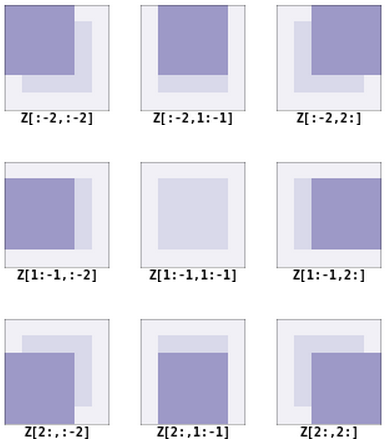
\includegraphics[scale=0.5]{../conway-slices.png}
\caption{Slicing ndarrays}
\end{figure}

What we actually did with the above code is to add all the darker blue
squares together. Since they have been chosen carefully, the result will
be exactly what we expected. If you want to convince yourself, consider
a cell in the lighter blue area of the central sub-figure and check what
will the result for a given cell.

    \subsection{Cell Iteration}\label{cell-iteration}

In a first approach, we can write the iterate function using the
\href{http://docs.scipy.org/doc/numpy/reference/generated/numpy.argwhere.html}{\texttt{argwhere}}
method that will give us the indices where a given condition is
\texttt{True}.

    \begin{Verbatim}[commandchars=\\\{\}]
{\color{incolor}In [{\color{incolor}40}]:} \PY{k}{def} \PY{n+nf}{iterate}\PY{p}{(}\PY{n}{Z}\PY{p}{)}\PY{p}{:}
             \PY{c}{\PYZsh{} Iterate the game of life : naive version}
             \PY{c}{\PYZsh{} Count neighbours}
             \PY{n}{N} \PY{o}{=} \PY{n}{np}\PY{o}{.}\PY{n}{zeros}\PY{p}{(}\PY{n}{Z}\PY{o}{.}\PY{n}{shape}\PY{p}{,} \PY{n+nb}{int}\PY{p}{)}
             \PY{n}{N}\PY{p}{[}\PY{l+m+mi}{1}\PY{p}{:}\PY{o}{\PYZhy{}}\PY{l+m+mi}{1}\PY{p}{,}\PY{l+m+mi}{1}\PY{p}{:}\PY{o}{\PYZhy{}}\PY{l+m+mi}{1}\PY{p}{]} \PY{o}{+}\PY{o}{=} \PY{p}{(}\PY{n}{Z}\PY{p}{[}\PY{l+m+mi}{0}\PY{p}{:}\PY{o}{\PYZhy{}}\PY{l+m+mi}{2}\PY{p}{,}\PY{l+m+mi}{0}\PY{p}{:}\PY{o}{\PYZhy{}}\PY{l+m+mi}{2}\PY{p}{]} \PY{o}{+} \PY{n}{Z}\PY{p}{[}\PY{l+m+mi}{0}\PY{p}{:}\PY{o}{\PYZhy{}}\PY{l+m+mi}{2}\PY{p}{,}\PY{l+m+mi}{1}\PY{p}{:}\PY{o}{\PYZhy{}}\PY{l+m+mi}{1}\PY{p}{]} \PY{o}{+} \PY{n}{Z}\PY{p}{[}\PY{l+m+mi}{0}\PY{p}{:}\PY{o}{\PYZhy{}}\PY{l+m+mi}{2}\PY{p}{,}\PY{l+m+mi}{2}\PY{p}{:}\PY{p}{]} \PY{o}{+}
                              \PY{n}{Z}\PY{p}{[}\PY{l+m+mi}{1}\PY{p}{:}\PY{o}{\PYZhy{}}\PY{l+m+mi}{1}\PY{p}{,}\PY{l+m+mi}{0}\PY{p}{:}\PY{o}{\PYZhy{}}\PY{l+m+mi}{2}\PY{p}{]}                \PY{o}{+} \PY{n}{Z}\PY{p}{[}\PY{l+m+mi}{1}\PY{p}{:}\PY{o}{\PYZhy{}}\PY{l+m+mi}{1}\PY{p}{,}\PY{l+m+mi}{2}\PY{p}{:}\PY{p}{]} \PY{o}{+}
                              \PY{n}{Z}\PY{p}{[}\PY{l+m+mi}{2}\PY{p}{:}  \PY{p}{,}\PY{l+m+mi}{0}\PY{p}{:}\PY{o}{\PYZhy{}}\PY{l+m+mi}{2}\PY{p}{]} \PY{o}{+} \PY{n}{Z}\PY{p}{[}\PY{l+m+mi}{2}\PY{p}{:}  \PY{p}{,}\PY{l+m+mi}{1}\PY{p}{:}\PY{o}{\PYZhy{}}\PY{l+m+mi}{1}\PY{p}{]} \PY{o}{+} \PY{n}{Z}\PY{p}{[}\PY{l+m+mi}{2}\PY{p}{:}  \PY{p}{,}\PY{l+m+mi}{2}\PY{p}{:}\PY{p}{]}\PY{p}{)}
             \PY{n}{N\PYZus{}} \PY{o}{=} \PY{n}{N}\PY{o}{.}\PY{n}{ravel}\PY{p}{(}\PY{p}{)}
             \PY{n}{Z\PYZus{}} \PY{o}{=} \PY{n}{Z}\PY{o}{.}\PY{n}{ravel}\PY{p}{(}\PY{p}{)}
         
             \PY{c}{\PYZsh{} Apply rules}
             \PY{n}{R1} \PY{o}{=} \PY{n}{np}\PY{o}{.}\PY{n}{argwhere}\PY{p}{(} \PY{p}{(}\PY{n}{Z\PYZus{}}\PY{o}{==}\PY{l+m+mi}{1}\PY{p}{)} \PY{o}{\PYZam{}} \PY{p}{(}\PY{n}{N\PYZus{}} \PY{o}{\PYZlt{}} \PY{l+m+mi}{2}\PY{p}{)} \PY{p}{)}
             \PY{n}{R2} \PY{o}{=} \PY{n}{np}\PY{o}{.}\PY{n}{argwhere}\PY{p}{(} \PY{p}{(}\PY{n}{Z\PYZus{}}\PY{o}{==}\PY{l+m+mi}{1}\PY{p}{)} \PY{o}{\PYZam{}} \PY{p}{(}\PY{n}{N\PYZus{}} \PY{o}{\PYZgt{}} \PY{l+m+mi}{3}\PY{p}{)} \PY{p}{)}
             \PY{n}{R3} \PY{o}{=} \PY{n}{np}\PY{o}{.}\PY{n}{argwhere}\PY{p}{(} \PY{p}{(}\PY{n}{Z\PYZus{}}\PY{o}{==}\PY{l+m+mi}{1}\PY{p}{)} \PY{o}{\PYZam{}} \PY{p}{(}\PY{p}{(}\PY{n}{N\PYZus{}}\PY{o}{==}\PY{l+m+mi}{2}\PY{p}{)} \PY{o}{|} \PY{p}{(}\PY{n}{N\PYZus{}}\PY{o}{==}\PY{l+m+mi}{3}\PY{p}{)}\PY{p}{)} \PY{p}{)}
             \PY{n}{R4} \PY{o}{=} \PY{n}{np}\PY{o}{.}\PY{n}{argwhere}\PY{p}{(} \PY{p}{(}\PY{n}{Z\PYZus{}}\PY{o}{==}\PY{l+m+mi}{0}\PY{p}{)} \PY{o}{\PYZam{}} \PY{p}{(}\PY{n}{N\PYZus{}}\PY{o}{==}\PY{l+m+mi}{3}\PY{p}{)} \PY{p}{)}
         
             \PY{c}{\PYZsh{} Set new values}
             \PY{n}{Z\PYZus{}}\PY{p}{[}\PY{n}{R1}\PY{p}{]} \PY{o}{=} \PY{l+m+mi}{0}
             \PY{n}{Z\PYZus{}}\PY{p}{[}\PY{n}{R2}\PY{p}{]} \PY{o}{=} \PY{l+m+mi}{0}
             \PY{n}{Z\PYZus{}}\PY{p}{[}\PY{n}{R3}\PY{p}{]} \PY{o}{=} \PY{n}{Z\PYZus{}}\PY{p}{[}\PY{n}{R3}\PY{p}{]}
             \PY{n}{Z\PYZus{}}\PY{p}{[}\PY{n}{R4}\PY{p}{]} \PY{o}{=} \PY{l+m+mi}{1}
         
             \PY{c}{\PYZsh{} Make sure borders stay null}
             \PY{n}{Z}\PY{p}{[}\PY{l+m+mi}{0}\PY{p}{,}\PY{p}{:}\PY{p}{]} \PY{o}{=} \PY{n}{Z}\PY{p}{[}\PY{o}{\PYZhy{}}\PY{l+m+mi}{1}\PY{p}{,}\PY{p}{:}\PY{p}{]} \PY{o}{=} \PY{n}{Z}\PY{p}{[}\PY{p}{:}\PY{p}{,}\PY{l+m+mi}{0}\PY{p}{]} \PY{o}{=} \PY{n}{Z}\PY{p}{[}\PY{p}{:}\PY{p}{,}\PY{o}{\PYZhy{}}\PY{l+m+mi}{1}\PY{p}{]} \PY{o}{=} \PY{l+m+mi}{0}
\end{Verbatim}

    Even if this first version does not use nested loops, it is far from
optimal because of the use of the 4 argwhere calls that may be quite
slow. We can instead take advantages of numpy features the following
way.

    \begin{Verbatim}[commandchars=\\\{\}]
{\color{incolor}In [{\color{incolor}41}]:} \PY{k}{def} \PY{n+nf}{iterate\PYZus{}2}\PY{p}{(}\PY{n}{Z}\PY{p}{)}\PY{p}{:}
             \PY{c}{\PYZsh{} Count neighbours}
             \PY{n}{N} \PY{o}{=} \PY{p}{(}\PY{n}{Z}\PY{p}{[}\PY{l+m+mi}{0}\PY{p}{:}\PY{o}{\PYZhy{}}\PY{l+m+mi}{2}\PY{p}{,}\PY{l+m+mi}{0}\PY{p}{:}\PY{o}{\PYZhy{}}\PY{l+m+mi}{2}\PY{p}{]} \PY{o}{+} \PY{n}{Z}\PY{p}{[}\PY{l+m+mi}{0}\PY{p}{:}\PY{o}{\PYZhy{}}\PY{l+m+mi}{2}\PY{p}{,}\PY{l+m+mi}{1}\PY{p}{:}\PY{o}{\PYZhy{}}\PY{l+m+mi}{1}\PY{p}{]} \PY{o}{+} \PY{n}{Z}\PY{p}{[}\PY{l+m+mi}{0}\PY{p}{:}\PY{o}{\PYZhy{}}\PY{l+m+mi}{2}\PY{p}{,}\PY{l+m+mi}{2}\PY{p}{:}\PY{p}{]} \PY{o}{+}
                  \PY{n}{Z}\PY{p}{[}\PY{l+m+mi}{1}\PY{p}{:}\PY{o}{\PYZhy{}}\PY{l+m+mi}{1}\PY{p}{,}\PY{l+m+mi}{0}\PY{p}{:}\PY{o}{\PYZhy{}}\PY{l+m+mi}{2}\PY{p}{]}                \PY{o}{+} \PY{n}{Z}\PY{p}{[}\PY{l+m+mi}{1}\PY{p}{:}\PY{o}{\PYZhy{}}\PY{l+m+mi}{1}\PY{p}{,}\PY{l+m+mi}{2}\PY{p}{:}\PY{p}{]} \PY{o}{+}
                  \PY{n}{Z}\PY{p}{[}\PY{l+m+mi}{2}\PY{p}{:}  \PY{p}{,}\PY{l+m+mi}{0}\PY{p}{:}\PY{o}{\PYZhy{}}\PY{l+m+mi}{2}\PY{p}{]} \PY{o}{+} \PY{n}{Z}\PY{p}{[}\PY{l+m+mi}{2}\PY{p}{:}  \PY{p}{,}\PY{l+m+mi}{1}\PY{p}{:}\PY{o}{\PYZhy{}}\PY{l+m+mi}{1}\PY{p}{]} \PY{o}{+} \PY{n}{Z}\PY{p}{[}\PY{l+m+mi}{2}\PY{p}{:}  \PY{p}{,}\PY{l+m+mi}{2}\PY{p}{:}\PY{p}{]}\PY{p}{)}
         
             \PY{c}{\PYZsh{} Apply rules}
             \PY{n}{birth} \PY{o}{=} \PY{p}{(}\PY{n}{N}\PY{o}{==}\PY{l+m+mi}{3}\PY{p}{)} \PY{o}{\PYZam{}} \PY{p}{(}\PY{n}{Z}\PY{p}{[}\PY{l+m+mi}{1}\PY{p}{:}\PY{o}{\PYZhy{}}\PY{l+m+mi}{1}\PY{p}{,}\PY{l+m+mi}{1}\PY{p}{:}\PY{o}{\PYZhy{}}\PY{l+m+mi}{1}\PY{p}{]}\PY{o}{==}\PY{l+m+mi}{0}\PY{p}{)}
             \PY{n}{survive} \PY{o}{=} \PY{p}{(}\PY{p}{(}\PY{n}{N}\PY{o}{==}\PY{l+m+mi}{2}\PY{p}{)} \PY{o}{|} \PY{p}{(}\PY{n}{N}\PY{o}{==}\PY{l+m+mi}{3}\PY{p}{)}\PY{p}{)} \PY{o}{\PYZam{}} \PY{p}{(}\PY{n}{Z}\PY{p}{[}\PY{l+m+mi}{1}\PY{p}{:}\PY{o}{\PYZhy{}}\PY{l+m+mi}{1}\PY{p}{,}\PY{l+m+mi}{1}\PY{p}{:}\PY{o}{\PYZhy{}}\PY{l+m+mi}{1}\PY{p}{]}\PY{o}{==}\PY{l+m+mi}{1}\PY{p}{)}
             \PY{n}{Z}\PY{p}{[}\PY{o}{.}\PY{o}{.}\PY{o}{.}\PY{p}{]} \PY{o}{=} \PY{l+m+mi}{0}
             \PY{n}{Z}\PY{p}{[}\PY{l+m+mi}{1}\PY{p}{:}\PY{o}{\PYZhy{}}\PY{l+m+mi}{1}\PY{p}{,}\PY{l+m+mi}{1}\PY{p}{:}\PY{o}{\PYZhy{}}\PY{l+m+mi}{1}\PY{p}{]}\PY{p}{[}\PY{n}{birth} \PY{o}{|} \PY{n}{survive}\PY{p}{]} \PY{o}{=} \PY{l+m+mi}{1}
             \PY{k}{return} \PY{n}{Z}
\end{Verbatim}

    Now, let's throw together a simple visualization for our Game of Life!
Don't worry about the \texttt{matplotlib} code, we'll deal with it
later.

    \begin{Verbatim}[commandchars=\\\{\}]
{\color{incolor}In [{\color{incolor}42}]:} \PY{k+kn}{import} \PY{n+nn}{matplotlib.pyplot} \PY{k+kn}{as} \PY{n+nn}{plt}
         \PY{k+kn}{from} \PY{n+nn}{matplotlib} \PY{k+kn}{import} \PY{n}{animation}
         \PY{k+kn}{from} \PY{n+nn}{IPython.display} \PY{k+kn}{import} \PY{n}{Image}
         \PY{o}{\PYZpc{}}\PY{k}{matplotlib} inline
\end{Verbatim}

    The cell below saves our animated Game of Life as a \texttt{.gif} format
on your computer.

    \begin{Verbatim}[commandchars=\\\{\}]
{\color{incolor}In [{\color{incolor}43}]:} \PY{n}{Z} \PY{o}{=} \PY{n}{np}\PY{o}{.}\PY{n}{random}\PY{o}{.}\PY{n}{randint}\PY{p}{(}\PY{l+m+mi}{0}\PY{p}{,}\PY{l+m+mi}{2}\PY{p}{,}\PY{p}{(}\PY{l+m+mi}{256}\PY{p}{,}\PY{l+m+mi}{256}\PY{p}{)}\PY{p}{)}
         \PY{n}{fig} \PY{o}{=} \PY{n}{plt}\PY{o}{.}\PY{n}{figure}\PY{p}{(}\PY{p}{)}
         \PY{n}{ax} \PY{o}{=} \PY{n}{plt}\PY{o}{.}\PY{n}{axes}\PY{p}{(}\PY{p}{)}
         
         \PY{n}{im} \PY{o}{=} \PY{n}{plt}\PY{o}{.}\PY{n}{imshow}\PY{p}{(}\PY{n}{Z}\PY{p}{,} \PY{n}{cmap}\PY{o}{=}\PY{l+s}{\PYZsq{}}\PY{l+s}{gray}\PY{l+s}{\PYZsq{}}\PY{p}{,} \PY{n}{interpolation}\PY{o}{=}\PY{l+s}{\PYZsq{}}\PY{l+s}{bicubic}\PY{l+s}{\PYZsq{}}\PY{p}{)}
         
         \PY{k}{def} \PY{n+nf}{updatefig}\PY{p}{(}\PY{o}{*}\PY{n}{args}\PY{p}{)}\PY{p}{:}
             \PY{n}{im}\PY{o}{.}\PY{n}{set\PYZus{}array}\PY{p}{(}\PY{n}{iterate\PYZus{}2}\PY{p}{(}\PY{n}{Z}\PY{p}{)}\PY{p}{)}
             \PY{k}{return} \PY{n}{im}\PY{p}{,}
             
         \PY{n}{ani} \PY{o}{=} \PY{n}{animation}\PY{o}{.}\PY{n}{FuncAnimation}\PY{p}{(}\PY{n}{fig}\PY{p}{,} \PY{n}{updatefig}\PY{p}{,} \PY{n}{interval}\PY{o}{=}\PY{l+m+mi}{200}\PY{p}{,} \PY{n}{blit}\PY{o}{=}\PY{n+nb+bp}{True}\PY{p}{)}
         
         \PY{n}{ani}\PY{o}{.}\PY{n}{save}\PY{p}{(}\PY{l+s}{\PYZsq{}}\PY{l+s}{demonstration.gif}\PY{l+s}{\PYZsq{}}\PY{p}{,} \PY{n}{writer}\PY{o}{=}\PY{l+s}{\PYZsq{}}\PY{l+s}{imagemagick}\PY{l+s}{\PYZsq{}}\PY{p}{,} \PY{n}{fps}\PY{o}{=}\PY{l+m+mi}{10}\PY{p}{)}
\end{Verbatim}

    \begin{center}
    \adjustimage{max size={0.9\linewidth}{0.9\paperheight}}{NumPy Basics_files/NumPy Basics_84_0.png}
    \end{center}
    { \hspace*{\fill} \\}
    
    And now, load up the \texttt{.gif} file with:

    \begin{Verbatim}[commandchars=\\\{\}]
{\color{incolor}In [{\color{incolor}44}]:} \PY{n}{Image}\PY{p}{(}\PY{n}{url}\PY{o}{=}\PY{l+s}{\PYZsq{}}\PY{l+s}{demonstration.gif}\PY{l+s}{\PYZsq{}}\PY{p}{)}
\end{Verbatim}

            \begin{Verbatim}[commandchars=\\\{\}]
{\color{outcolor}Out[{\color{outcolor}44}]:} <IPython.core.display.Image object>
\end{Verbatim}
        
    \section{Lab: Gradient Descent}\label{lab-gradient-descent}

For those of you who have taken linear algebra, or have dealt with
problems involving solutions to systems of linear equations such as

\begin{align*}
a_{1,1}x_1 + a_{1,2}x_2 + \cdots + a_{1,n}x_n &= b_1 \\
a_{2,1}x_1 + a_{2,2}x_2 + \cdots + a_{2,n}x_n &= b_2 \\
\vdots& \\
a_{n,1}x_1 + a_{n,2}x_2 + \cdots + a_{n,n}x_n &= b_n \\
\end{align*}

you might be familiar with Gaussian elimination, which provides a
systematic way to find a solution, if one exists. Now, we can compactly
write this system of equations as a \emph{matrix-vector} equation
$A\vec{x}=\vec{b}$, where \[(A_{i,j})=a_{i,j},\]
\[\vec{x}=(x_1, x_2, \cdots, x_n)^T,\] and
\[\vec{b}=(b_1, b_2, \cdots, b_n)^T.\]

\subsection{Problems with Gaussian
Elimination}\label{problems-with-gaussian-elimination}

Gaussian elimination has some significant advantages. First off, it will
always find a solution, if one exists, in a finite number of steps. This
is a powerful property, but it comes at a cost. For an $n\times n$
matrix $A$, Gaussian elimination is an $\mathcal{O}(n^3)$ algorithm,
which means that the number of steps required to solve the system is
proportional to the \textbf{cube} of the number of rows or columns of
the matrix.

This isn't so bad for an $2\times 2$ matrix, but it is downright
impossible for an $10000\times 10000$ one. So, we need to find a better
approach.

\subsection{Theory for Gradient
Descent}\label{theory-for-gradient-descent}

One alternative is the \emph{method of gradient descent}. Consider a
function
\[f(\vec{x})=\frac{1}{2}\vec{x}^T A \vec{x} - \vec{b}^T\vec{x} + c,\]
where $A$ is a symmetric matrix, and $c$ is a scalar constant. Now, this
implies that $f : \mathbb{R}^n \to \mathbb{R}$, which means that $f$ is
a scalar function of $n$ variables.

Specifically, $f$ is a \emph{quadratic} function, and it has a minimum.
One can show that gradient of $f$ is given by
\[ \nabla f(\vec{x}) = A\vec{x} - \vec{b}\] for symmetric matrices $A$.
This means that by finding an $\vec{x}$ that satisfies
$\nabla f(\vec{x})=0$ will simultaneously solve the system of equations
$A\vec{x}=\vec{b}$.

You can visualize $f$ as a quadratic bowl, and the method of gradient
descent looks for the minimum of the bowl.

In the above image, we have the paraboloid formed by $f$, as well as the
iterations of solutions given by the gradient descent algorithm.
Alternatively, you can think about the contours of $f$, and for this you
can think of gradient descent as updating the locations of the guesses
in the following image.

Now, the gradient of a function points in the direction of
greatest-initial increase of the function. Perhaps mysteriously, the
\emph{antigradient}, $-\nabla f$ points in the direction of
greatest-initial \emph{decrease} of $f$. So, to minimize $f(\vec{x})$,
we can follow $-\nabla f$ all the way down until we reach the bottom of
the bowl.

\subparagraph{Note:}\label{note}

From here on out, $\vec{x}$ and $\vec{b}$ will \emph{always} denote
vectors, so we will not include the $\vec{\cdot}$ notation.

\subsection{Constructing the
algorithm}\label{constructing-the-algorithm}

Suppose $x$ is the solution to the equation $Ax=b$. Imagine that you're
given a \emph{guess} solution $x_{(i)}$. Then the \emph{residual}
between the ideal solution and the guess is given by
\[r_{(i)} = b - Ax_{(i)}.\] Coincidentally,
$r_{(i)}=-\nabla f(x_{(i)})$, which means that when we update to
$x_{(i+1)}$ we want to move in the direction of $r_{(i})$.

So, when we update to $x_{(i+1)}$, we will update according to the rule
\[x_{(i+1)} = x_{(i)} + \alpha r_{(i)},\] where $\alpha$ is some number.

What should $\alpha$ be? We want to choose $\alpha$ that makes the
biggest improvement in one single step. It turns out that after doing
some calculations, this $\alpha$ is given by
\[ \alpha = \frac{r_{(i)}^T r_{(i)}}{r_{(i)}^T A r_{(i)}}. \]

\subsubsection{Gradient Descent
Pseudocode}\label{gradient-descent-pseudocode}

Suppose you are given a matrix $A$ that is square and symmetric, along
with a vector $b$. Here is how Gradient Descent works:

\begin{enumerate}
\def\labelenumi{\arabic{enumi}.}
\itemsep1pt\parskip0pt\parsep0pt
\item
  Set $i=0$.
\item
  Initialize $x_0$.
\item
  Set $r_i = b - Ax_i$.
\item
  Let $\alpha = \dfrac{r_i^Tr_i}{r_i^TAr_i}$
\item
  Set $x_{i+1} = x_i + \alpha r_i$.
\item
  Increment $i$.
\item
  Go back to step (3).
\end{enumerate}

\subsubsection{Terminating the
algorithm}\label{terminating-the-algorithm}

When $f(x_{(i)})$ is very close to the minimum, the vector $x_{(i)}$ is
very close to the solution $x$. So, the residual vector $r_{(i)}$ is
very close to the zero vector. In other words, the \emph{magnitude} of
$r_{(i)}$ is approximately 0.

We can use this to build a terminating condition. Since the magnitude of
$r_{(i)}$ is given by \[\|r_{(i)}\| = r_{(i)}^Tr_{(i)},\] we can tell
our algorithm to stop as soon as $\|r_{(i)}\|$ is below some error
tolerance.

\subsection{Try It!}\label{try-it}

We are now going to build and test an algorithm that applies the
gradient descent method. Use the Gradient Descent Pseudocode to build a
gradient descent algorithm. Remember, this function will take a
symmetric matrix and a vector as inputs.

\subsubsection{Test}\label{test}

Try testing your algorithm with the matrices:
$A = \begin{bmatrix} 3 & 2 \\ 2 & 6 \\ \end{bmatrix}$ and
$b = \begin{bmatrix} 2 \\ -8\\ \end{bmatrix}$ Your algorithm should
produce: $x = \begin{bmatrix} 2 \\ -2 \end{bmatrix}$

\subsubsection{Real Test}\label{real-test}

Now it is time to test your algorithm with an arbitrary large matrix.
First, we have to generate a large matrix

\begin{Shaded}
\begin{Highlighting}[]
\KeywordTok{def} \NormalTok{generate_large_matrix(n):}
    \NormalTok{A = np.random.random_intergers(-}\DecValTok{100}\NormalTok{,}\DecValTok{100}\NormalTok{,(n,n)) }\CommentTok{# Generate a square matrix with int entries in [-100,100]}
    \NormalTok{A = A.T.dot(A) }\CommentTok{#Makes a matrix symmetric}
    \NormalTok{A[A<}\DecValTok{0}\NormalTok{] = }\DecValTok{0} \CommentTok{#Makes all matrix entries positive}
    \KeywordTok{return} \NormalTok{A}
\end{Highlighting}
\end{Shaded}

Now we have to generate a vector

\begin{Shaded}
\begin{Highlighting}[]
\KeywordTok{def} \NormalTok{generate_vector(n):}
    \NormalTok{b = np.random.random_intergers(-}\DecValTok{100}\NormalTok{,}\DecValTok{100}\NormalTok{,n)}
    \KeywordTok{return} \NormalTok{b}
\end{Highlighting}
\end{Shaded}

Input the generated matrix and vector into your algorithm. (Make sure
that the $n$ for the large matrix is the same as the $n$ for the
vector.)

Did it work? (Hopefully, yes.)


    % Add a bibliography block to the postdoc
    
    
    
    \end{document}
